\documentclass[10pt,letterpaper]{article}
\usepackage[margin=0.75in,columnsep=0.25in]{geometry}
\usepackage[T1]{fontenc}
\usepackage{lmodern}
\usepackage{amsmath,amssymb}
\usepackage{graphicx,booktabs,tabularx,array}
\usepackage[round,authoryear]{natbib}
\usepackage{placeins}
\usepackage{xurl}
\usepackage[hidelinks]{hyperref}
\setlength{\parindent}{1em}
\setlength{\parskip}{0pt}
\setlength{\textfloatsep}{11pt plus 3pt minus 2pt}
\setlength{\floatsep}{9pt plus 2pt minus 2pt}
\setlength{\intextsep}{10pt plus 2pt minus 2pt}
\setlength{\emergencystretch}{1em}
\renewcommand{\topfraction}{0.93}
\renewcommand{\dbltopfraction}{0.93}
\renewcommand{\textfraction}{0.05}
\setcounter{dbltopnumber}{3}
\newcommand{\cfmoa}{CF-MoA}
\newcommand{\sysL}{MedRAG-Llama}
\newcommand{\sysQ}{MedRAG-Qwen}
\newcommand{\pct}{\%}
\graphicspath{{figures/}}
\begin{document}
\twocolumn[{
\begin{center}
{\LARGE\bfseries CF-MoA: Taxonomy-Guided Benchmarking and Agent\\[3pt]
Orchestration for Counterfactual Medical Reasoning\par}
\vspace{10pt}
{\large Anonymous Authors}\\[9pt]
\end{center}
\begin{center}\begin{minipage}{0.95\textwidth}
\begin{abstract}
Medical question answering requires selective responses to changing evidence: a new finding can justify an additional treatment, invalidate an earlier recommendation, reorder competing diagnoses, or leave a conclusion unchanged. We introduce a five-relation functional taxonomy that connects these behaviors across heterogeneous tasks and guides the design of specialized reasoning operations. From 11 sources, we construct a benchmark of 6,104 units and 13,000 target judgments, preserving native task interfaces and source-specific scoring. Evaluating seven medical question-answering configurations reveals recurring weaknesses in support updating and candidate comparison that aggregate accuracy obscures. We address these weaknesses with a counterfactual mixture of agents (\cfmoa{}): five functional roles for support addition, support removal, candidate comparison, model-based consequence calculation, and stable readout, organized by a sparse controller. On this development benchmark, the corresponding heads improve all 21 comparisons across seven configurations and three support-update and candidate-comparison categories. The complete controller raises the aggregate score of two MedRAG configurations from 48.20 to 58.29 and from 47.35 to 59.36, with gains on both answer-changing and answer-preserving pairs. Component controls identify explicit support execution and catalog-based re-decision as useful mechanisms. The taxonomy, benchmark, and controller connect behavioral diagnosis to concrete operations for improving counterfactual medical reasoning.

\end{abstract}
\smallskip
\end{minipage}\end{center}
\vspace{7pt}
}]
\section{Introduction}
\label{sec:introduction}

A medical answer depends on the evidence that supports it. When a patient's condition changes, a system may need to add a newly indicated treatment, withdraw an option whose prerequisites no longer hold, or reconsider the leading diagnosis. Other changes should leave the answer intact. Selective updating requires tracking how the changed information bears on the particular judgment being requested.

Consider a treatment supported by two independent indications. Removing one indication leaves the other available to justify treatment; withdrawing the treatment requires checking both support paths. A diagnostic update requires a different operation: new evidence can strengthen a candidate while another diagnosis remains more likely. The final answer's change or preservation captures the outcome of these decisions. The underlying operation---adding support, removing support, or comparing alternatives---explains what the system must compute.

Retrieval-augmented generation (RAG) gives medical language models access to external knowledge, and agent-based systems add iterative retrieval, multiple answers, or explicit control of reasoning \citep{xiong2024medrag,li2026medrgag,wu2026marag,jiang2025tcrag}. Using that evidence requires an appropriate decision procedure for the requested update. Existing counterfactual, perturbation, and robustness resources test complementary aspects of this ability through different units, answer spaces, and evaluation rules. A shared behavioral vocabulary can connect their observations while preserving their original tasks.

We introduce a taxonomy of five functional relations between a change and a target judgment: support addition, support removal, candidate comparison, consequence calculation, and target preservation. The categories can overlap: the same change may add evidence for a candidate and require a new comparison among alternatives. We use this taxonomy to organize an inventory of 26 candidate resources and construct a benchmark spanning 11 sources. Its 6,104 evaluation units retain the native questions, options, target definitions, and source-specific scoring definitions.

Functional evaluation reveals weaknesses hidden by aggregate rankings. Seven configurations from six system families achieve aggregate scores between 47.35 and 51.61, while their scores on support removal range from 7.59 to 41.77. Different systems lead on different functional categories. These profiles motivate an operation-centered approach: identify the computation required by the observed failure mode, then attach a component that performs it through the existing interface.

We organize these components as a counterfactual mixture of agents (\cfmoa{}), with five functional roles. Its support agents execute three-valued rules, its comparison agent makes an explicit decision over a diagnosis catalog, its consequence agent applies local interventions to a supplied executable model, and its preservation agent stabilizes native answers through structured readout. A sparse controller selects the applicable operation from the visible input and available capabilities. This design gives each agent a concrete responsibility and allows compatible operations to share an implementation.

Our contributions are threefold. First, we introduce a functional taxonomy and a provenance-preserving benchmark that connect diverse medical counterfactual and robustness tasks. Second, we provide a seven-configuration diagnostic evaluation, together with head-level comparisons that improve all 21 system--category combinations on support addition, support removal, and candidate comparison. Third, we develop \cfmoa{} and evaluate the complete adopted controller on two MedRAG configurations, obtaining aggregate gains of 10.09 and 12.01 percentage points and improved correctness on both changing and preserving pairs. The accompanying controls explain which operations account for these improvements and when further aggregation adds little value.

\section{Related Work}
\label{sec:related-work}

\paragraph{Behavioral evaluation and counterfactual tests.}
Behavioral testing organizes evaluation around capabilities and expected responses to controlled changes. CheckList combines linguistic capabilities with minimum functionality, invariance, and directional tests \citep{ribeiro2020checklist}. Contrast sets probe local decision boundaries through small, meaningful edits that typically change the reference label \citep{gardner2020contrastsets}. Dynabench develops this diagnostic perspective through human-and-model-in-the-loop data collection \citep{kiela2021dynabench}. These approaches motivate evaluating the relationship between an input change and its required response. Our five-category taxonomy applies that perspective to medical tasks: it records the changed condition, the requested decision, and the evidence needed to justify revision or preservation. Categories can overlap when one case requires several operations. This gives a shared interpretation to tests drawn from sources with different task formats.

\paragraph{Medical counterfactual and robustness benchmarks.}
Medical datasets expose several distinct consequences of perturbing an input. MedEinst changes discriminative evidence to test differential diagnosis \citep{chen2026medeinst}, while MedPIC-Bench provides patient-specific medication questions with counterfactual task families \citep{medpicbench}. HIV treatment scenarios examine causal consistency across interventions, interactions, and side effects \citep{prosperi2026hiv}. Counterfactual Patient Variations and DiversityMedQA examine demographic sensitivity in clinical decisions \citep{benkirane2025bias,rawat2024diversitymedqa}; cultural-cue perturbations and AMQA extend this line to cultural context and adversarial medical questions \citep{rezaei2026cultural,xiao2025amqa}. MedPerturb varies gender cues, language style, and presentation format \citep{gourabathina2025medperturb}. MedCounterFact studies how models follow supplied medical evidence when its content conflicts with plausibility or safety \citep{mo2026faithfulness}. MedRGB and BioRAB assess retrieval conditions, including misleading or counterfactual evidence \citep{ngo2024medrgb,li2025biorab}. We bring eligible instances from these eleven sources into one benchmark while preserving their native questions, answer spaces, and reference relations. The resulting functional labels connect heterogeneous perturbations to the reasoning operation that each instance actually tests.

\paragraph{Medical RAG.}
Retrieval-augmented generation combines a language model with external information \citep{lewis2020rag}. MIRAGE and the MedRAG toolkit examine how corpora, retrievers, and language models affect medical question answering \citep{xiong2024medrag}. MedRGAG connects retrieved and parametric knowledge \citep{li2026medrgag}; MA-RAG uses multiple rounds of agentic retrieval and reasoning \citep{wu2026marag}. MedGENIE supplies generated contexts for medical questions \citep{frisoni2024medgenie}, and TC-RAG maintains a memory stack to control iterative retrieval \citep{jiang2025tcrag}. These methods provide complementary ways to acquire and organize knowledge. Our seven evaluated configurations use them to diagnose which functional requirements remain difficult, then test operation-specific heads on the resulting outputs and admissible evidence. This connects system-level evaluation to targeted repairs such as recalculating support and comparing diagnostic candidates.

\paragraph{Agent aggregation.}
Self-consistency aggregates answers across sampled reasoning paths \citep{wang2023selfconsistency}, while Mixture-of-Agents passes multiple agents' outputs between successive layers \citep{wang2025moa}. Contextual calibration addresses prompt-dependent answer preferences \citep{zhao2021calibrate}. These ideas motivate distinct controls for additional sampling, candidate comparison, and aggregation. MedGuideX transforms executable guideline logic into factual and counterfactual supervision for post-training medical models \citep{shen2026medguidex}. Our support agents execute guideline logic during inference to recompute a current answer. CF-MoA gives its five agents explicit functional responsibilities and combines their outputs through a shared input contract and routing interface. Our evaluation follows both the gains from integrating these specialized operations and the incremental effects of candidate verification, tying each system change to the behavior it is intended to improve.

\section{A Functional Benchmark for Medical Counterfactual Reasoning}
\label{sec:benchmark}

We organize medical counterfactual tasks around the relationship between a change and a specified judgment. A \emph{comparison unit} links a source-provided variant to its reference or identifies an explicit within-question hypothetical. A \emph{target judgment} identifies what is being assessed within that unit. This distinction lets a single clinical narrative support several functional annotations while retaining the source's original question and answer contract. The resulting taxonomy covers condition changes, hypothetical evidence, and perturbations whose effects are evaluated through native task performance.
% Evidence: docs/data/classification.md, annotation contract and target-level definitions;
% docs/paper/research_dossier.md, Sections 3.1--3.2.

\subsection{Five overlapping functional relations}

\textbf{R1: adding support.} A change introduces identifiable evidence for a target judgment. For example, newly reported wheezing can support a bronchitis candidate without establishing it as the unique diagnosis. \textbf{R2: withdrawing support.} An identifiable basis for a judgment becomes invalid; the annotation states which basis is lost and preserves any independent support. \textbf{R3: comparing alternatives.} A change requires reassessing the relative support for at least two identifiable candidates. Replacing a history of spontaneous pneumothorax with deep-vein thrombosis illustrates a change relevant to the comparison between pneumothorax and pulmonary embolism in MedEinst~\cite{chen2026medeinst}. \textbf{R4: deriving consequences.} A changed premise requires propagating an established relationship to an outcome not directly supplied. \textbf{R5: preserving a judgment.} A real change leaves the evidence relevant to a specified target intact; the annotation gives a reason for that invariance.
% Evidence: docs/data/classification.md, definitions and retained examples;
% cited MedEinst examples are locally retained source cases 10000 and 13249.

These relations overlap because they describe functions at the target level. The same observation may add support to one diagnosis and alter its comparison with another. Annotation therefore records the change, target, applicable relations, supporting text, and conclusions that cannot be inferred, then takes the union of target labels for the parent unit. Omission of a symptom does not establish its explicit absence, and an unchanged answer alone does not establish invariance. Native comparison axes are preserved: an internal hypothetical and an externally edited patient attribute receive separate treatment when they address different judgments.
% Evidence: docs/data/classification.md, comparison-axis and cannot_infer rules.

\subsection{Collection, qualification, and sampling}

We registered 26 candidate sources and obtained 15, comprising 14 text resources and one multimodal metadata release lacking required images. Their normalized archive contains 55,991 units. Source acquisition, semantic classification, and scoring eligibility are recorded separately. Qualification requires the source materials needed to answer the native task and an established scoring interface. This process yielded an eligible pool of 38,123 units and 77,781 target judgments from 11 sources. The included resources cover diagnostic and prescribing edits~\cite{chen2026medeinst,medpicbench}, treatment hypotheticals~\cite{prosperi2026hiv}, demographic and cultural perturbations~\cite{benkirane2025bias,rezaei2026cultural,xiao2025amqa,rawat2024diversitymedqa}, clinical-service judgments~\cite{gourabathina2025medperturb}, hypothetical research evidence~\cite{mo2026faithfulness}, and evidence robustness~\cite{ngo2024medrgb,li2025biorab}.
% Evidence: docs/data/sources.md; docs/data/construction.md;
% paper_story_alignment/benchmark_contribution_audit.json.

Language-model agents performed structured semantic annotation and review, supported by cross-checks and targeted audits. The construction pipeline preserves provenance and explicit correction history. Review distinguishes whether a functional relation holds from whether its reference answer supports scoring. For example, a valid invariance annotation can remain while an unreliable reference is excluded from scoring. Targeted review corrected 172 judgments across 130 units; these corrections are retained alongside their earlier versions. Unit identifiers, source locations, eligibility decisions, and target-to-input mappings make the final evaluation traceable to the acquired materials.
% Evidence: docs/data/construction.md, review corrections;
% docs/paper/research_dossier.md, Section 3.3.

The frozen v5 evaluation retains all eligible R1--R4 targets and samples 450 R5 units without replacement from each of eight sources. Sampling uses sorted source-specific identifiers and a fixed seeded procedure, without consulting model predictions. Original semantic labels remain available, while a separate evaluation-label field specifies membership in this evaluation. This yields 6,104 unique comparison units, with category counts of 2,866/79/733/13/3,600 for R1--R5. Category memberships overlap; in particular, all 733 R3 units also belong to R1. Equal R5 allocations preserve source coverage while reducing the much larger invariance pool.
% Evidence: frozen v5 sampling_protocol.json and source_summary.csv;
% docs/data/construction.md, v5 sampling; dossier Sections 3.4--3.5.

\subsection{Native inputs and scoring}

The selected units contain 13,000 target judgments and materialize into 13,905 distinct model inputs, including reference endpoints. Each method has 15,616 native scoring mappings: one input may support multiple targets, and shared references can serve several units. Models receive the current question, native options, required evidence, and output contract. Reference and variant endpoints are answered independently; gold answers, functional labels, annotation rationales, and the opposite endpoint's answer remain outside inference.
% Evidence: docs/evaluation/protocol.md, Sections 2.1 and 5.1.

Native interfaces preserve the distinctions between sources. MedEinst requires open diagnosis, MedPIC uses multiple-answer selection, and MedPerturb expands eligible visit, management, and resource judgments separately. Hypothetical research evidence remains attached to its relation question. MedRGB retains the locally frozen six evidence conditions, with the fully relevant condition serving as the reference endpoint. Under our evaluation protocol, systems may additionally retrieve external evidence according to their configured permissions; this combines fixed perturbed evidence with dynamic retrieval.
% Evidence: docs/evaluation/protocol.md, native format preservation and MedRGB conditions.

For unit $u$, let $\mathcal{J}_u$ contain its eligible non-reference native scoring mappings and let $c_j\in\{0,1\}$ denote primary correctness. We report
\begin{equation}
 s_u=\frac{1}{|\mathcal{J}_u|}\sum_{j\in\mathcal{J}_u}c_j,
 \qquad
 \mathrm{ALL}=\frac{1}{|\mathcal{U}|}\sum_{u\in\mathcal{U}}s_u,
 \label{eq:native-score}
\end{equation}
where $|\mathcal{U}|=6{,}104$. Category scores apply the same aggregation to their eligible members and mappings. Tables report these scores as percentages. Thus, ALL weights comparison units equally, rather than averaging category percentages or pooling all model inputs.

Scoring retains native choice keys, multi-answer sets, relation labels, and frozen diagnosis normalization. Invalid outputs and unresolved protocol failures stay in the denominator. We additionally distinguish variant correctness, answer agreement, and both-endpoints-correct performance. The last measure requires successful answers on both sides, making it useful for evaluating whether systems respond to relevant changes while preserving correct judgments under irrelevant ones. These functional strata provide the diagnostic basis for the specialized operations introduced next.
% Evidence: docs/evaluation/protocol.md, native scoring and failure policy.

\section{CF-MoA: Sparse Orchestration of Five Functional Roles}
\label{sec:method}

CF-MoA implements five functional agent roles: adding support (A1), withdrawing support (A2), comparing candidates (A3), deriving consequences (A4), and preserving task-relevant judgments (A5). These roles correspond to R1--R5 and operate through a sparse controller. The adopted configuration, denoted B, selects an applicable operation from the current input's capabilities and returns a native answer (Figure~\ref{fig:architecture}). The base system supplies its current answer and actual inference context; agents share backbone weights and, where applicable, deterministic components.
% Evidence: docs/research/cf_moa.md, adopted_B_five_operations_v1;
% docs/paper/research_dossier.md, Section 5.9.

\subsection{Capability routing and native readout}

The controller selects operations by task format and available resources. Its fixed priority routes diagnosis-format inputs to A3, eligible rule tasks to the shared A1/A2 kernel, inputs providing a complete executable model to A4, and supported single-choice, robustness, or relation tasks with saved original messages to A5. Other inputs retain the base response. Routing uses visible options and question structure alongside format and resource availability; source identifiers, benchmark relation labels, gold answers, and paired endpoints are excluded. Capability-based routing allows a component developed on one functional subset to operate on compatible inputs elsewhere in the benchmark.

Each role operates within a defined domain: finite prescribing rules for A1/A2, a fixed diagnosis catalog for A3, a supplied executable mechanism and state for A4, and supported native decision formats for A5. In the complete v5 evaluation, each backbone routes 3,560 inputs to A3, 123 to A1/A2, 10,178 to A5, and 44 to passthrough. A4 has no qualifying clinical v5 input; its supplied-model evaluation is reported separately. The controller records the selected route, requests, operation traces, and complete returned response.
% Evidence: five_agent_framework_audit.json; complete v5 coverage in
% docs/research/cf_moa_experiment_report.md, Sections 16.6--16.13.

\subsection{A1/A2: scoped support recomputation}

A1 and A2 recompute support with a shared kernel of 71 manually encoded rules drawn from selected recommendations in the 2023 American Geriatrics Society Beers Criteria~\citep{ags2023beers}. Eligibility checks require a supported multiple-choice format, an age of at least 65 in the implemented question pattern, and a recognized medication option. The kernel identifies the requested action and scope, such as avoidance or renal dose adjustment. One call to the original backbone extracts the required patient facts and evidence sentence identifiers from the numbered current question. The extraction input excludes the base answer and retrieved documents. Missing or rejected evidence produces an unknown value.
% Evidence: docs/research/r2_support_head.md, execution guide Sections 2--3.

The executor evaluates conditions, exceptions, and independent support paths using \textsc{met}, \textsc{contradicted}, and \textsc{unknown}. Conjunction combines requirements within a path; disjunction preserves independent paths. Consequently, invalidating one risk does not remove an option supported by another satisfied risk. Let $S_0$ be the initial valid option set and let $M,C,U$ partition options by their aggregate status. A1 adds $M\setminus S_0$; A2 removes $C\cap S_0$. For ordinary valid sets, the result is
\begin{equation}
 S^{\star}=M\cup(S_0\cap U).
 \label{eq:support-update}
\end{equation}
The native assembler additionally handles exclusive ``None'' options, invalid initial answers, and empty outputs. Both roles therefore use one fact extraction and one execution, while retaining separate addition and withdrawal traces.
% Evidence: docs/research/cf_moa.md, minimal five-operation B;
% docs/research/r2_support_head.md, three-valued execution and assembly.

\subsection{A3: catalog-based candidate comparison}

A3 compares all 49 disease names in the public DDXPlus catalog~\cite{ddxplus}. The same backbone reads the current patient and the base system's actual context, with diagnoses bound to scoreable codes under six fixed catalog orders. For each order, it subtracts a content-free log-score prior from the patient-conditioned code score, following the general calibration principle of separating contextual evidence from answer preferences~\cite{zhao2021calibrate}. The prior is the logarithm of the mean of three content-free candidate distributions, computed separately for each order; its subtraction coefficient is fixed at one. A3 selects the highest corrected score per order and votes across orders, breaking vote ties using average corrected probabilities. The selected catalog entry is mapped back to the native diagnosis. The catalog supplies candidates for this decision stage; the scorer uses its separate, frozen normalization dictionary.
% Evidence: docs/research/r3_candidate_comparison.md, retained catalog/calibration;
% r3_catalog_calibration.py and r3_catalog_distribution_head.py.

\subsection{A4: executing a local intervention}

A4 compiles an intervention into a typed local patch and executes it to compute its consequences. Its input supplies the executable model, parameters, complete initial state, and factual action schedule. The patch preserves all unmodified actions. The numerical executor runs factual and patched trajectories from the same starting state and projects their consequences onto the requested time and outcome. Our implementation uses the public glucose--insulin simulator~\cite{simglucose}. Local patches reduce the need to regenerate a complete action plan, allowing intervention fidelity to be evaluated against a same-tool full-plan control. The returned consequence follows from the supplied mechanism and executed actions.
% Evidence: docs/research/r4_consequence_head.md, typed-patch delivery and
% frozen 24-profile validation; source simulator dependency is cited above.

\subsection{A5: task-adapted robust readout}

A5 implements task-adapted robust readout through component F. For ordinary supported tasks, F preserves the complete original messages and samples up to five native responses at temperature $0.7$, seeds 42--46, and a 2,048-token output limit. It votes over valid answer keys, stops once one key receives three votes, and returns the earliest complete response carrying a winning key. Final vote ties use earliest occurrence; if no vote is valid, the first response remains invalid. This adapts sampling and answer aggregation to the native output contract~\cite{wang2023selfconsistency}.

For explicit premise--hypothesis tasks with two polarity options, F uses a natural language inference (NLI) branch. It scores both A/B label mappings directly, generates one current-question analysis, and scores both mappings again conditioned on that analysis. Each two-label distribution is normalized before the four semantic distributions are averaged. The highest mean determines the answer; exact ties follow native option order. A final model call generates the complete native response with its answer field constrained to that decision. This path uses four one-token score callbacks and two complete generations at temperature zero, preserving the original evidence and required auxiliary fields. Missing code scores require a matching score request and remain visible in the cost ledger.
% Evidence: docs/research/r5_invariance_head.md, independent combination interface;
% Documents/Codex/2026-09-18/r5_head/delivery/r5_head.py, optimize/decide_paths.

\begin{figure*}[t]
\centering
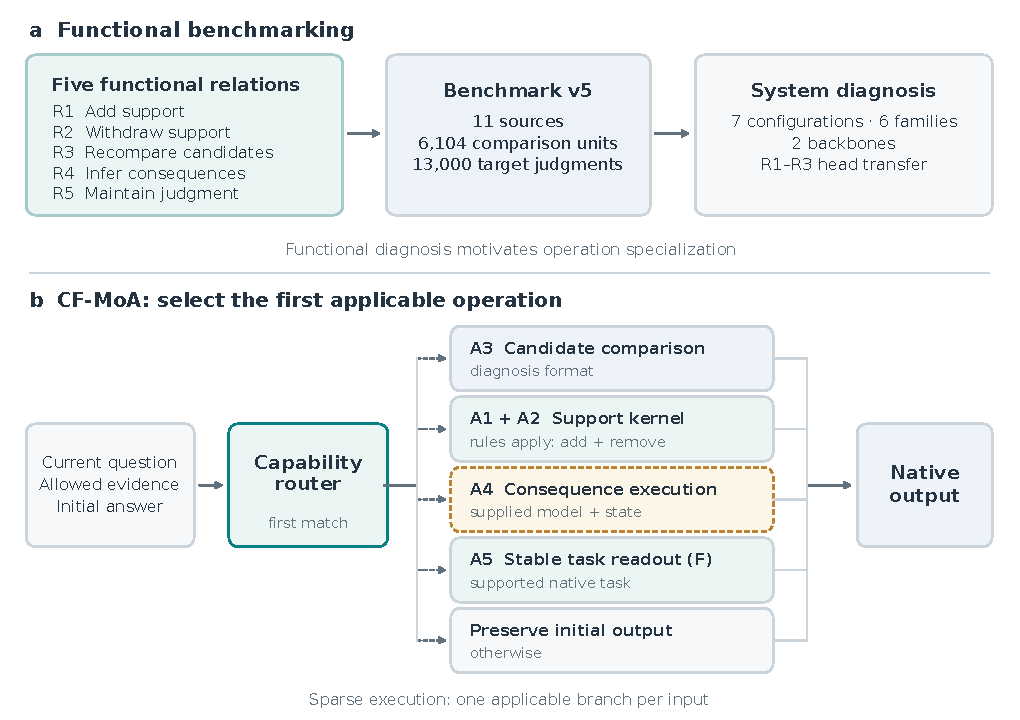
\includegraphics[width=\textwidth]{cf_moa_architecture.pdf}
\caption{From functional diagnosis to agent orchestration. The benchmark describes five relations between a change and a target judgment. CF-MoA implements the corresponding operations through a sparse controller: support addition and removal share a rule executor, candidate comparison uses a diagnosis catalog, consequence calculation requires an executable model, and stable readout handles the remaining eligible interfaces. Routing uses the current input and available capabilities; A4 is evaluated separately on supplied-model tasks.}
\label{fig:architecture}
\end{figure*}
\section{Experimental Setup}
\label{sec:experimental_setup}

\subsection{Seven-system baseline comparison}
\label{sec:experimental_setup-model-configurations-and-controls}

The formal v5 comparison uses M0 direct answering, M2 MedRGAG with the local all-Llama
adaptation, M3 MA-RAG in its intrinsic configuration, M4 MedRAG--Llama, M5 MedRAG--Qwen,
M6 MedGENIE version 2, and M7 TC-RAG with the selected typed-control version 2. M0, M2,
M4, and M6 use Llama-3.1-8B-Instruct; M3, M5, and M7 use Qwen3-8B
\citep{dubey2024llama,yang2025qwen3}. Thus, seven configurations span six baseline
families and two underlying backbones. MA-RAG generates eight solver candidates per
round for at most four rounds, with early stopping on agreement. MedRGAG, MedGENIE,
and TC-RAG are the documented local adaptations, rather
than claims of exact reproduction of every published model and resource setting.

Each selected configuration covers the same 13,905 unique inputs and 15,616 scoring
mappings. Coverage combines new predictions with strictly matched historical reuse where
available: M0 reuses 8,877 and generates 5,028 predictions; M2 reuses 6,687 and generates
7,218; M3 reuses 3,690 and generates 10,215. M4--M7 each have 13,905 new predictions in
their selected complete run. Full coverage therefore means complete evaluated outputs,
not seven simultaneous runs from scratch. Invalid and unaccepted terminal outputs remain
in the common denominator.

The selected M4 baseline includes structured-output repair, whereas M5 retains its earlier
unconstrained output protocol. Corpora, upstream procedures, and budgets also vary across
families. Cross-system differences compare these concrete settings and cannot all be
assigned to an isolated algorithm or backbone effect. M1, an earlier MedRGAG initial
retrieval control, and the superseded i-MedRAG implementation are historical experiments,
not additional completed v5 configurations (Appendix~\ref{sec:appendix_development}).

\subsection{Seven-system terminal-head evaluation}
\label{sec:experimental_setup-terminal-heads}

We evaluate the frozen terminal heads on every member of R1, R2, and R3 for all seven
configurations. In R1, each configuration routes 1,780 diagnostic inputs to catalog
re-decision and 72 prescribing inputs to rules, retaining the other 1,014 answers. R3
contains 680 catalog inputs, 10 rule inputs, and 43 retained single-choice answers. R2
covers 55 of 79 inputs with rules and retains the remaining 24. Uncovered inputs remain
in their category denominators.

Diagnostic scores are generated with each configuration's actual original context and
backbone; earlier completed scores and exactly identical requests are reused as recorded.
The fact extractor sees the current question, options, and required fields, but no
method-specific retrieved history or initial answer. Consequently, its two backbone-specific
fact sets can be fixed and combined offline with seven original-answer sets. This is a
valid comparison of seven terminal systems, while the rule branch is not seven newly
executed upstream retrieval pipelines. No backbone is substituted to improve another
system's head result.

We compare the diagnostic head with single-pass catalog selection and uncorrected voting.
For R2, a constant ``none'' control intervenes on the same 55 inputs and preserves each
original answer on the other 24. Remaining-support correctness is reported alongside its
total. Additional same-facts execution, question-scope, and external-source evaluations
are kept within their original experimental scopes. The original formal baseline scores
and the development head scores remain separate tables.

\subsection{Two-configuration CF-MoA composition and verification}
\label{sec:experimental_setup-cf-moa}

The later six-arm experiment uses only the two MedRAG configurations M4 and M5, with
Qwen thinking disabled. Within each configuration, all six arms share the same frozen
full-v5 input scope and original contexts. It tests the composition of established heads
with further operations, followed by additional candidate verification; it does not
extend the six-arm experiment to all seven systems.

The ordinary F readout uses bfloat16 weights, temperature 0.7, top-p 1.0, a 2,048-token
output budget, and a 131,072-token context limit under the saved vLLM 0.8.5 profiles. The
F readout uses structured native output in both configurations. The existing catalog and
fact-extraction components retain their own shorter-context, temperature-zero profiles.
Exact per-component settings, prompts, code snapshots, and reuse bindings remain in the
released experiment package. The experiments use inference and deterministic tools; no new
model training is reported.

Table~\ref{tab:arms} summarizes the six evaluation arms.

\begin{table}[htbp]
\centering
\small
\caption{Six evaluation arms. C1 and B denote the same adopted operation core.}
\label{tab:arms}
\setlength{\tabcolsep}{5pt}
\begin{tabularx}{\linewidth}{@{}lXX@{}}
\toprule
Arm & Decision rule & Role in the comparison \\
\midrule
C0 & Original MedRAG configuration & Original-system reference \\
C1 / B & Adopted operation core & Strong system baseline \\
C2 & B plus candidate-only binary verification & Same-pool verification without saved rationales \\
C3 & B plus rationale-conditioned binary verification & Main research extension \\
C4 & B with old F votes plus three additional answers & Expanded-pool sampling control \\
C5 & B plus joint selection over the same candidates and rationales & Alternative same-pool selection control \\
\bottomrule
\end{tabularx}
\end{table}


C4 uses the predefined supplementary seeds 42, 43, and 44 on eligible ordinary-F
disagreements. A failed required supplementary answer leaves the control unavailable,
rather than silently converting it into a two-draw control. C5 scores a joint finite-code
choice under two opposing code assignments. C2, C3, and C5 preserve the existing pool.
Their comparisons share the original computation but have different additional request and
prompt costs; none is described as equal-cost merely because a common budget ceiling
exists.

Complete v5 is the scope of this later experiment. Earlier 121-input and 52-input
development panels informed its design and are not independent confirmation sets. The older 52-input
panel still lacks four original M5 C0 outputs; that historical gap does not affect the
complete full-v5 C0 results reported here. No new model calls or native grading are
performed for this manuscript; the figures and tables are rebuilt from frozen completed
results.

\subsection{Failure retention and computation
accounting}
\label{sec:experimental_setup-failure-retention-and-computation-accounting}

All arms retain the complete input and native-unit denominators. An unavailable answer
counts against performance under the frozen contract and is also reported explicitly. We
separate a valid but incorrect answer, an unavailable answer, and a verifier failure with
a retained F answer. Pool-trigger coverage includes the full scope and is not filtered by
subsequent success or gold correctness.

For the later composition experiment, per-method computation assigns the shared B computation once to each independently
considered B-based method, then adds that method's own incremental requests. This
estimates the attributable computation of a method assembled from the recorded components.
It is distinct from the physical ledger for the multi-arm experiment, where shared calls
were actually executed once. Exact cache reuse is not treated as free historical
computation. The upstream C0 and retrieval costs, and some historical event times, remain
unknown. Reported event seconds are not exclusive GPU hours, end-to-end latency, or energy
measurements.

\section{Results}
\label{sec:results}

\subsection{Functional evaluation exposes different weaknesses}
\label{sec:baseline_results}
% Generated from frozen audited summaries by build_paper_figures.py.
\begin{table*}[t]
\centering
\small
\setlength{\tabcolsep}{5.5pt}
\caption{Complete v5 results for seven baseline configurations and two CF-MoA instantiations. Scores are percentages of native-unit means; bold denotes the highest value in each column.}
\label{tab:main-system-results}
\begin{tabular}{llrrrrrr}
\toprule
System & Backbone & ALL & R1 & R2 & R3 & R4 & R5 \\
\multicolumn{2}{l}{\emph{Comparison units}} & 6,104 & 2,866 & 79 & 733 & 13 & 3,600 \\
\midrule
Direct & Llama & 48.10 & 30.04 & 8.86 & 17.87 & 38.46 & 65.70 \\
MedRGAG & Llama & 48.81 & 31.33 & 7.59 & 24.69 & 53.85 & 65.88 \\
MA-RAG & Qwen & 51.61 & 26.73 & 34.18 & 8.59 & 38.46 & \textbf{73.37} \\
MedRAG & Llama & 48.20 & 27.84 & 29.11 & 30.42 & 53.85 & 65.28 \\
MedRAG & Qwen & 47.35 & 28.58 & 41.77 & 25.24 & 53.85 & 63.42 \\
MedGENIE & Llama & 48.02 & 29.94 & 18.99 & 21.42 & \textbf{61.54} & 65.15 \\
TC-RAG & Qwen & 49.43 & 31.44 & 29.11 & 28.92 & 30.77 & 66.17 \\
\midrule
\textbf{CF-MoA (B)} & Llama & 58.29 & 44.63 & 48.10 & 53.21 & 53.85 & 68.84 \\
\textbf{CF-MoA (B)} & Qwen & \textbf{59.36} & \textbf{46.62} & \textbf{58.23} & \textbf{60.03} & 23.08 & 68.79 \\
\bottomrule
\end{tabular}
\par\smallskip
\begin{minipage}{0.97\textwidth}\footnotesize Each configuration covers 13,905 unique inputs. ALL averages non-reference task scores within units and then across units; R labels may overlap. Llama denotes Llama-3.1-8B-Instruct and Qwen denotes Qwen3-8B. The selected MedRAG-Llama baseline includes its output repair.\end{minipage}
\end{table*}


The seven baselines occupy a narrow range on the aggregate metric but exhibit substantially different functional profiles (Table~\ref{tab:main-system-results}). MA-RAG has the highest baseline aggregate score, 51.61, and the highest preservation score, 73.37, yet scores 8.59 on candidate comparison. \sysQ{} leads the baselines on support removal at 41.77, while \sysL{} leads on candidate comparison at 30.42. Direct answering reaches 48.10 overall but only 8.86 on support removal. Thus, a system can answer many ordinary or preservation-oriented items correctly while struggling to revise the support for a specific decision.

The taxonomy makes these differences actionable. Support removal calls for checking whether an answer's prerequisites still hold; diagnosis calls for comparing viable candidates under the changed evidence. Neither need is fully described by the number of retrieved passages or generated answers. This distinction motivates the specialized operations evaluated next.

\subsection{Specialized heads transfer across seven configurations}
\label{sec:head_results}
\begin{figure*}[t]
\centering
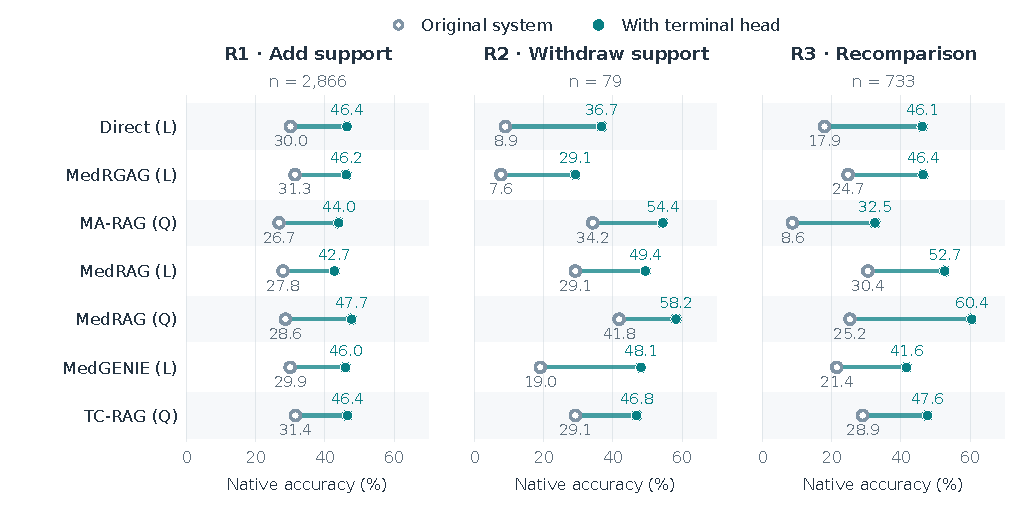
\includegraphics[width=\textwidth]{seven_system_head_gains.pdf}
\caption{Original and head-augmented performance across all seven configurations. Each panel uses the complete corresponding category: support addition ($n=2{,}866$), support removal ($n=79$), and candidate comparison ($n=733$). All 21 comparisons improve. Category memberships overlap; exact correct counts and branch coverage are in Appendix~\ref{app:heads}.}
\label{fig:seven-head-gains}
\end{figure*}

Figure~\ref{fig:seven-head-gains} shows improvements in all 21 system--category comparisons. Support addition rises from an original range of 26.73--31.44\% to 42.74--47.70\%; support removal rises from 7.59--41.77\% to 29.11--58.23\%; and candidate comparison rises from 8.59--30.42\% to 32.47--60.44\%. The gains occur across direct answering, retrieval-based systems, and systems with their own agent or control loops. They show that a functional head can repair failures left by different upstream workflows.

The head construction reflects the overlap between categories. On support addition, the adopted wrapper routes 1,780 units to diagnosis, 72 to rule execution, and retains the original result on 1,014 units. On candidate comparison, 680 units use diagnosis, ten use rules, and 43 retain their original result. These shared operations connect the category analysis to an implementable system, while avoiding a separate learned model for every label.

\paragraph{Candidate presentation accounts for much of the diagnosis gain.}
On the 680-unit diagnostic subset, averaging across the seven systems, the original score is 20.97\%, a single catalog decision reaches 45.44\%, six uncalibrated decisions reach 46.47\%, and calibrated decisions reach 46.13\%. The largest common improvement therefore comes from asking the model to make an explicit decision over the available diagnoses. Additional voting and calibration have smaller, configuration-dependent effects. For \sysL{}, the correct count changes from 203 to 339 with one catalog decision and to 359 with either six-decision variant. For \sysQ{}, the corresponding counts are 160, 382, 402, and 410. Appendix~\ref{app:heads} gives every configuration and additional source checks.

\paragraph{Both support operations contribute.}
% Generated from frozen audited summaries by build_paper_figures.py.
\begin{table}[t]
\centering
\small
\setlength{\tabcolsep}{6pt}
\caption{Support-operation ablation on all 123 rule inputs, reusing the same extracted facts and execution states. Parentheses give the change in correct outputs relative to the complete kernel.}
\label{tab:support-ablation}
\begin{tabular}{lrr}
\toprule
Policy & Llama & Qwen \\
\midrule
Full support kernel & 69/123 & 71/123 \\
Without add & 43/123 (-26) & 48/123 (-23) \\
Without remove & 53/123 (-16) & 60/123 (-11) \\
\bottomrule
\end{tabular}
\par\smallskip
\begin{minipage}{\linewidth}\footnotesize A1 and A2 share one rule kernel. Unavailable outputs remain in the denominator.\end{minipage}
\end{table}

The shared support executor uses the extracted facts to add newly justified options and remove contradicted ones. On the 123-input control in Table~\ref{tab:support-ablation}, disabling addition reduces correct answers from 69 to 43 for Llama and from 71 to 48 for Qwen. Disabling removal reduces them to 53 and 60. Both operations contribute under the same fact extraction and rule statuses.

The small support-removal category also exposes a dataset prior: a coverage-matched constant ``None'' control obtains more correct answers than the head in each of the seven configurations. The head's value is therefore better assessed together with the operation ablation and the nine covered prescribing examples with remaining support, where the constant control scores zero. On these nine examples, five configurations improve, one is unchanged, and one declines. This result favors explicit support execution as a useful operation while showing why the raw category average alone is an incomplete diagnosis.

\subsection{The complete controller improves overall and paired correctness}
\label{sec:full_results}

On the complete benchmark, the aggregate score rises from 48.20 to 58.29 for \sysL{} and from 47.35 to 59.36 for \sysQ{} (Table~\ref{tab:main-system-results}). The gains are 10.09 percentage points (95\% family bootstrap interval: 8.96--11.23) and 12.01 points (10.92--13.15). Both configurations improve on support addition, support removal, candidate comparison, and preservation. Their final scores also exceed the highest aggregate baseline, although the within-configuration contrasts provide the direct measure of the controller's effect.

On the 13 clinical consequence units, \sysL{} remains at 53.85 while \sysQ{} decreases from 53.85 to 23.08 under the readout branch. This localized regression is retained in the main table alongside the larger-category gains.

\begin{figure*}[t]
\centering
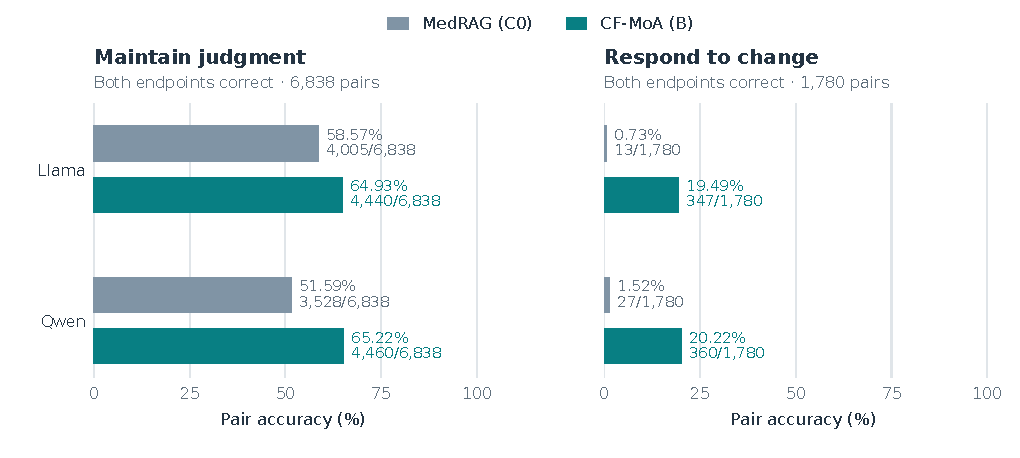
\includegraphics[width=\textwidth]{paired_behavior.pdf}
\caption{Correctness on both members of a pair. On answer-preserving pairs, correct counts increase from 4,005 to 4,440 for Llama and from 3,528 to 4,460 for Qwen ($n=6{,}838$). On answer-changing pairs, they increase from 13 to 347 and from 27 to 360 ($n=1{,}780$). Agreement alone does not satisfy either measure.}
\label{fig:paired-behavior}
\end{figure*}

Paired evaluation tests the behavior that motivates the benchmark (Figure~\ref{fig:paired-behavior}). On answer-preserving pairs, both-side correctness rises from 58.57 to 64.93\% for Llama and from 51.59 to 65.22\% for Qwen. On answer-changing pairs, it rises from 0.73 to 19.49\% and from 1.52 to 20.22\%, respectively. All four paired differences have positive family-bootstrap intervals. The controller thus improves selective response to a change as well as correctness under a change that should leave the answer intact. The lower absolute scores on changing pairs identify evidence-sensitive updating as a continuing challenge.

\subsection{Conditional execution and stable readout}
\label{sec:conditional}

The consequence agent addresses tasks with an explicit executable model. On 24 virtual physiological profiles with 12 questions each, typed local intervention produces correct binary and numerical outputs on all 288 questions for both backbones. A same-tools alternative that asks the model to generate a complete plan obtains 270 and 222 correct numerical outputs. Removing the intervention from the patch procedure reduces numerical correctness to 67 for both backbones. These controls support the value of a constrained local edit followed by execution in the supplied model (Appendix~\ref{app:model}).

Stable readout is evaluated on a separate 208-group component panel combining answer sampling and NLI interfaces. Its group-weighted paired score improves from 60.19 to 65.90\% for Llama and from 59.17 to 66.47\% for Qwen. In the final 16-group extension, both-side correctness improves from 11 to 12 groups and from 12 to 13 groups relative to the matched single-answer control. These observations motivated its use as the broad readout branch of the adopted controller.

\subsection{More aggregation is not uniformly better}
\label{sec:extensions}

We evaluated further aggregation on the same full input set. A rationale-conditioned verifier scores the distinct candidates already present in the saved readout pool and returns an existing complete answer. Relative to B, it changes the aggregate score by $-1.81$ points for Llama and $+0.93$ points for Qwen. Its candidate-only and joint-selection counterparts likewise do not provide a consistent improvement over B; three additional sampled answers yield 58.32 and 59.67, with more unavailable outputs. The complete six-arm comparison is retained in Appendix~\ref{app:full}. Earlier generated-answer aggregation also underperformed the adopted controller on its development panel. These results support sparse execution of useful operations as the default \cfmoa{} design.

The controller adds measurable computation. Attributed component requests total 59,800 for Llama and 58,301 for Qwen, before the original answering and retrieval costs. Rationale-conditioned verification adds 13,308 and 9,820 requests. This cost and its mixed gains make it a less attractive default than the adopted controller; Appendix~\ref{app:cost} gives the physical request and token accounting.

\FloatBarrier
\section{Discussion}
\label{sec:discussion}

The seven-system results establish that terminal decision procedures can improve a
range of medical question-answering systems under a common native evaluation contract.
The benefit is not confined to the two MedRAG configurations: direct answering,
MedRGAG, MA-RAG, MedGENIE, and TC-RAG also improve throughout the three declared
development strata. Preserving these results alongside their controls is necessary to
understand the research outcome. Mixed contributions from calibration, or incomplete
external validation, do not erase the measured gain of the complete terminal head.

What changes depends on the task. The diagnostic component provides an explicit answer
space and a new original-model decision; the rule component executes support conditions
and combines them with the original answer. These are distinct interventions, and R1's
reuse of R2/R3 components demonstrates useful transfer across support requirements
without constituting three independent algorithms. A common component can also preserve
method differences through the original context, UNKNOWN inheritance, and fallback.
The evidence supports system improvement with explicit attribution limits, rather than
a claim that all failures share one cause.

The later CF-MoA core combines the catalog, rules, and repeated readout in two
configurations. Its improvement concerns that broader composition and its additional
computation. It neither replaces the seven-system findings nor extends the full CF-MoA
result to five untested configurations. The composition's gain also cannot be reassigned
to candidate verification introduced afterward.

Additional candidate verification poses a distinct selection problem. By design, C3 cannot
recover an answer key absent from its pool, and it can replace a correct selected answer
with an incorrect existing candidate. The repair and damage counts establish that
successful and harmful switches both occur; they do not measure the frequency of missing
correct candidates or diagnose the medical cause of each mistake. Pool quality and
selector quality should therefore be measured separately. Enlarging the pool is also not
automatically beneficial: the C4 control changes both candidate opportunity and failure
exposure, with its unavailable outputs retained in the result.

Rationales provide extra information to the verifier, but they can contain unsupported
statements or persuasive explanations for a wrong key. Their positive incremental point
estimates over C2 justify further study of how they affect selection. They do not certify
rationale truthfulness, establish calibrated confidence, or guarantee improvement over
majority-based readout. A direct evaluation of rationale validity and an independent
replication of pool generation would be needed to test those stronger interpretations.

The source and pair analyses constrain the use of an aggregate gain. A positive overall
score can coexist with harm on a particular source, and a changed overall mean can coexist
with unchanged respond-pair performance. No arm was selected separately for each source or
backbone after inspecting these outcomes. Keeping the adopted core as the common default
preserves the distinction between an observed local gain and a deployment or
generalization decision.

Finally, the five-role description is useful only when tied to actual computation. Shared
rule addition and removal are two functions of one execution. A model-based executor with
zero coverage cannot explain a clinical benchmark gain. Recording these facts makes the
architecture interpretable without implying that every question benefits from five-agent
collaboration.

\section{Limitations}
\label{sec:limitations}

\textbf{Development exposure and confirmation.} The full v5 benchmark was already exposed
and contributed to method development and selection. Current bootstrap intervals do not
remove that exposure. A planned frozen-method evaluation on new families and a second
independently generated F pool were deferred and have not been executed. The manuscript
therefore provides no independently confirmed generalization or across-pool stability
result.

\textbf{Scope and scoring.} The sources differ in task semantics, patient realism,
perturbation construction, and reference quality. R labels overlap, some groups are small,
and the 13-unit R4 clinical subset has especially limited coverage. Classification follows
the project's documented target-level review rules; no clinician inter-annotator agreement
estimate is reported. Canonical diagnostic matching can penalize clinically related
wording, while source expected answers do not provide a new clinical adjudication. An
empty list of newly established data defects in the final closeout is not evidence that
all items and labels have undergone a complete expert medical review.

\textbf{Attribution and model comparison.} B combines several already developed components
with additional resources and inference. Only specified local comparisons, such as the
rule-operation ablation and C3 versus C2, isolate narrower design changes. M4 and M5
differ in output protocol as well as model. Their disagreement in C3's effect is
configuration dependence; a pure backbone explanation requires matched-protocol
experiments. Candidate-trigger membership also differs because each model generates its
own pool.

\textbf{Clinical applicability.} This is an offline benchmark study, not a prospective
patient study, treatment trial, or deployment evaluation. Rule coverage is limited, and
the A4 physiological results concern a supplied mathematical model. Neither exact-match
improvements nor successful model execution establish clinical safety or correctness
outside those contracts.

\textbf{Computation and reproducibility.} Some original-system costs and historical
timings are unknown. Shared-call attribution describes the measured components rather than
complete end-to-end resource use. The figure package reproduces reported summaries and can
check them against the released compressed result records; it does not rerun the full
language-model experiment. Original input data, licenses, model access, retrieval indices,
and environment-specific paths remain separate prerequisites for fresh inference.

\FloatBarrier
\bibliographystyle{plainnat}
\bibliography{references}
\clearpage
\onecolumn
\appendix
\section{Benchmark Composition and Annotation}
\label{app:benchmark}

\subsection{Source inventory and qualification}
Table~\ref{tab:story-benchmark} gives the exact composition of the frozen evaluation. Source citations and acquisition records accompany the source manifest. The original inventory contained 26 candidates, of which 15 were acquired. Four acquired resources did not contribute eligible v5 targets: the clinical laboratory and EquityMedQA resources required additional answer or rubric adjudication; MedCF required an editing operation outside the implemented answering protocol; and MedMKEB lacked the required images. For the other 11 candidates, the specified fixed cases, counterfactual edits, or required restricted context had not been obtained at collection time.

The 55,991 archived units comprise 53,494 text units and 2,497 metadata units with missing images. An initial review frame contained 28,243 units and 80,910 judgments. Its review ledger records 603 individual semantic reviews, 13,464 grouped semantic reviews, and 14,176 structural checks. Subsequent completion and eligibility review covered all archived units, producing 109,599 reviewed judgments, of which 77,781 were eligible in 38,123 units. The evaluation sample is drawn from this completed pool.

% Generated by scripts/build_story_assets.py from frozen audited summaries.
\begin{table}[tb]
\centering
\small
\setlength{\tabcolsep}{4pt}
\caption{Complete v5 benchmark composition by source. R1--R5 columns count units bearing each category label.}
\label{tab:story-benchmark}
\resizebox{\linewidth}{!}{%
\begin{tabular}{llrrrrrrr}
\toprule
ID & Source & Units & Judgments & R1 & R2 & R3 & R4 & R5 \\
\midrule
M01 & MedEinst & 1,780 & 2,816 & 1,780 & 0 & 680 & 0 & 0 \\
M02 & MedPIC-Bench & 167 & 182 & 96 & 75 & 10 & 0 & 0 \\
M06 & HIV causal scenarios & 13 & 13 & 0 & 0 & 0 & 13 & 0 \\
M10 & CPV-MedQA & 451 & 451 & 1 & 0 & 0 & 0 & 450 \\
M11 & Counterfactual Cultural Cues & 517 & 517 & 67 & 0 & 0 & 0 & 450 \\
M12 & FairMedQA/AMQA & 584 & 584 & 134 & 0 & 43 & 0 & 450 \\
M14 & DiversityMedQA & 454 & 454 & 0 & 4 & 0 & 0 & 450 \\
M17 & MedPerturb & 450 & 1,344 & 0 & 0 & 0 & 0 & 450 \\
M20 & MedCounterFact & 788 & 1,720 & 788 & 0 & 0 & 0 & 450 \\
M22 & MedRGB & 450 & 4,469 & 0 & 0 & 0 & 0 & 450 \\
M23 & BioRAB & 450 & 450 & 0 & 0 & 0 & 0 & 450 \\
\midrule
\textbf{Total} &  & 6,104 & 13,000 & 2,866 & 79 & 733 & 13 & 3,600 \\
\bottomrule
\end{tabular}}
\par\smallskip
\begin{minipage}{\linewidth}\footnotesize The benchmark contains 6,104 unique units and 13,000 target judgments. Category memberships overlap and must not be summed as independent units. Target judgments are distinct from the 13,905 inference inputs and 15,616 native scoring mappings per system. The separate supplied-model A4 panel is not added to this table.\end{minipage}
\end{table}


\subsection{Annotation examples and overlap}
An annotation identifies the source comparison axis before assigning a relation. In a MedEinst case, the addition of wheezing supports a bronchitis candidate (R1), while the associated diagnostic question can require comparison with acute laryngitis (R3). A DiversityMedQA sex-attribute change removes one demographic basis for a Lesch--Nyhan candidate (R2), while other findings remain available. In CPV-MedQA, changing an ethnicity description leaves the chemotherapy and ototoxicity evidence relevant to a pharmacological question intact (R5). Each label describes a relation between a specified change and its target in the full case context.

Labels are assigned to targets and then combined at the unit level. In v5, R3 is contained in R1; R1 and R5 share 450 units, R1 and R2 share four, and R2 and R3 share three. R1--R3 contain 2,941 distinct units. The sum of category memberships is 7,291, whereas the union used for ALL contains 6,104 units. The 13,000 selected target judgments, 13,905 distinct inputs, and 15,616 scoring mappings refer to different representations of these same tasks. Of the scoring mappings, 6,818 address reference endpoints and 8,798 address non-reference endpoints.

\subsection{Sampling and version lineage}
The earlier v2 evaluation contained 3,105 units and eight sources. A v3 display assigned overlapping units to a single category for presentation, preserving their answers. The completed v4 pool restored multi-label evaluation and expanded eligibility review. The v5 evaluation used in this paper retains all eligible R1--R4 targets and samples 450 R5 units from each of eight sources. These source samples are drawn without replacement from sorted identifiers using a source-specific seeded procedure. The original semantic labels and the selected evaluation labels are stored separately. Eligibility and seeded sampling determine membership independently of predictions and method scores.

The 450-unit allocation balances source representation within R5, with sampling fractions defined by each source's eligible pool. Related variants remain linked to their parent families for paired analysis and bootstrap resampling. The source manifest, membership files, and scoring mappings define the evaluated sample.
\FloatBarrier

\section{Component Evidence and Controls}
\label{app:heads}

\subsection{Complete head comparisons}
Table~\ref{tab:seven-heads} reports correct counts for every configuration in the head comparison. The R1 wrapper uses diagnosis on 1,780 units, support rules on 72, and the saved original answer on 1,014. R2 uses rules on 55 units and preserves 24 original answers. R3 uses diagnosis on 680 units, rules on ten, and preserves 43 original answers. These are unit-level coverage counts for the head experiment; the full controller's input-level coverage additionally includes reference endpoints and other compatible tasks.

% Generated from existing archived head outcomes; correct counts.
\begin{table}[tb]
\centering
\small
\caption{Archived original $\rightarrow$ head correct counts on R1--R3 for all seven configurations. The head combines candidate re-decision with rule support and preserves original answers outside coverage. These are analyses of exposed development data, using saved method-context decisions and shared backbone-level rule facts; they are not seven new upstream pipeline reruns. R3 is contained in R1; the three sets contain 2,941 distinct units.}
\label{tab:seven-heads}
\begin{tabular*}{\linewidth}{@{\extracolsep{\fill}}lrrr@{}}
\toprule
System & R1 ($n=2{,}866$) & R2 ($n=79$) & R3 ($n=733$) \\
\midrule
M0 Direct & $861 \rightarrow 1,329$ & $7 \rightarrow 29$ & $131 \rightarrow 338$ \\
M2 MedRGAG & $898 \rightarrow 1,323$ & $6 \rightarrow 23$ & $181 \rightarrow 340$ \\
M3 MA-RAG & $766 \rightarrow 1,260$ & $27 \rightarrow 43$ & $63 \rightarrow 238$ \\
M4 MedRAG--L & $798 \rightarrow 1,225$ & $23 \rightarrow 39$ & $223 \rightarrow 386$ \\
M5 MedRAG--Q & $819 \rightarrow 1,367$ & $33 \rightarrow 46$ & $185 \rightarrow 443$ \\
M6 MedGENIE & $858 \rightarrow 1,317$ & $15 \rightarrow 38$ & $157 \rightarrow 305$ \\
M7 TC-RAG & $901 \rightarrow 1,331$ & $23 \rightarrow 37$ & $212 \rightarrow 349$ \\
\bottomrule
\end{tabular*}
\end{table}

% Generated from archived controls; all cells are correct counts.
\begin{table}[tb]
\centering
\small
\caption{Controls expose limits of attributing the head gains. (a) R3 diagnosis subset ($n=680$): original, one catalog order (order 0), majority across catalog orders without calibration, and calibrated majority. Calibration does not improve every system. (b) R2 ($n=79$): the same-coverage None control predicts None on 55 covered inputs and preserves 24 original answers. Its higher aggregate score reflects 46 covered None targets; it misses all nine covered cases with remaining support. The last two columns isolate these nine cases.}
\label{tab:head-controls}
\textbf{(a) R3: correct out of 680}\par\smallskip
\begin{tabular*}{\linewidth}{@{\extracolsep{\fill}}lrrrr@{}}
\toprule
System & Original & Order 0 & Majority & Calibrated \\
\midrule
M0 Direct & 116 & 299 & 314 & 314 \\
M2 MedRGAG & 163 & 320 & 325 & 315 \\
M3 MA-RAG & 33 & 215 & 200 & 204 \\
M4 MedRAG--L & 203 & 339 & 359 & 359 \\
M5 MedRAG--Q & 160 & 382 & 402 & 410 \\
M6 MedGENIE & 137 & 296 & 288 & 276 \\
M7 TC-RAG & 186 & 312 & 324 & 318 \\
\bottomrule
\end{tabular*}
\medskip
\textbf{(b) R2: aggregate and remaining-support subset}\par\smallskip
\begin{tabular*}{\linewidth}{@{\extracolsep{\fill}}lrrrr@{}}
\toprule
System & Head /79 & None /79 & Head /9 & None /9 \\
\midrule
M0 Direct & 29 & 48 & 6 & 0 \\
M2 MedRGAG & 23 & 47 & 4 & 0 \\
M3 MA-RAG & 43 & 58 & 3 & 0 \\
M4 MedRAG--L & 39 & 58 & 4 & 0 \\
M5 MedRAG--Q & 46 & 56 & 6 & 0 \\
M6 MedGENIE & 38 & 52 & 5 & 0 \\
M7 TC-RAG & 37 & 54 & 2 & 0 \\
\bottomrule
\end{tabular*}
\end{table}


\subsection{Diagnosis: catalog, calibration, and source checks}
The public catalog contains 49 diagnoses, while the frozen task scorer recognizes 46 normalized diagnosis keys. The fixed public catalog is supplied to the decision component independently of the current item's gold answer. On 680 diagnostic units, Table~\ref{tab:head-controls}(a) separates the single-catalog improvement from repeated selection and calibration. Across repaired R3 outcomes, 1,186 of 1,272 previously failed outputs were unmapped diagnoses, 23 were otherwise invalid, and 63 were valid wrong answers. This breakdown indicates that output grounding accounts for a large part of the measured improvement. The task scorer treats unmapped outputs as incorrect.

Additional controls explored alternative name/code presentations on 40 diagnostic inputs. Direct code selection with a 384-token budget obtained 18/21 correct for Llama/Qwen; direct name selection at a 128-token budget obtained 15/18. Reasoning with names at 384 tokens obtained 18/19, while reasoning with codes at that budget obtained 21/22. The direct-name/direct-code comparison jointly varies representation and token budget. The evidence ledger retains the complete run identities and budgets.

Two additional source checks assessed catalog compatibility. On 47 ASCENT records, the calibrated head obtained 38/39 correct for Llama/Qwen, compared with 39/39 for uncalibrated voting and 38/39 for a single catalog decision. These records included 42 source-training and five source-test examples and subsequently informed development. Across three CUPCase batches totaling 18 records, the calibrated head obtained 15/16, uncalibrated voting 16/17, single selection 15/18, and character-length-normalized candidate likelihood 15/14. Catalog-based selection performs well on these additional records; calibration provides no consistent incremental advantage.

\subsection{Support removal and remaining support}
The constant ``None'' control in Table~\ref{tab:head-controls}(b) uses the same 55-input rule coverage and retains the same 24 original answers outside coverage. Forty-six covered targets have ``None'' as their answer; the other nine retain support for at least one option. On those nine, original correct counts for Direct, MedRGAG, MA-RAG, MedRAG-Llama, MedRAG-Qwen, MedGENIE, and TC-RAG are 5/4/1/3/0/2/3, and head counts are 6/4/3/4/6/5/2. This subset measures the ability to retain independent support after another basis is removed.

The 123-input add/remove ablation in the main text holds the extracted facts and statuses fixed. It evaluates the shared executor on the controller's complete rule-input panel, which extends beyond the 79-unit R2 category. The full executor leaves one Llama input and 14 Qwen inputs unavailable; these remain included in the 123-input denominator. The contrast tests the effect of the specified operations under the same upstream extraction.

\subsection{Supplied-model consequence execution}
\label{app:model}
The separate model panel uses 24 virtual parameter and initial-state profiles, each with 12 questions. A question supplies the physiological mechanism, factual schedule, requested local intervention, and output projection. The typed-patch procedure edits the named action and executes the resulting trajectory. The full-plan control has the same tool access but regenerates a complete plan; the no-intervention control retains patch structure while omitting the actual intervention. Table~\ref{tab:historical_model} reports binary, numerical, and full-output correctness for the 288 structured queries over these virtual profiles.

\begin{table}[htbp]
\centering
\small
\caption{Historical explicit-model validation. Each configuration contains 288 questions from 24
virtual parameter/initial-state profiles. Counts report correct outputs within the
supplied model contract.}
\label{tab:historical_model}
\setlength{\tabcolsep}{5pt}
\begin{tabularx}{\linewidth}{@{}lXrrr@{}}
\toprule
Config. & Historical arm & \shortstack{Binary\\/288} & \shortstack{Numerical\\/288} & \shortstack{Full output\\/288} \\
\midrule
M4 & Ordinary reanswer & 118 & 0 & 0 \\
M4 & Full execution & 286 & 270 & 270 \\
M4 & Patch without intervention execution & 234 & 67 & 67 \\
M4 & Typed patch and execution & 288 & 288 & 288 \\
\addlinespace
M5 & Ordinary reanswer & 187 & 0 & 0 \\
M5 & Full execution & 265 & 222 & 222 \\
M5 & Patch without intervention execution & 234 & 67 & 67 \\
M5 & Typed patch and execution & 288 & 288 & 288 \\
\bottomrule
\end{tabularx}
\end{table}


\subsection{Stable readout and generated aggregation}
The F component panel comprises an initial 64 groups, an additional 128 groups, and a final frozen extension of 16 groups. Group-weighted paired scores for the complete 208-group panel are reported in Section~\ref{sec:conditional}. The ordinary branch aggregates valid native answer keys; the NLI branch combines direct and analysis-conditioned semantic probabilities across both label mappings. The component's exact stopping, tie-breaking, and invalid-output policies are specified in Section~\ref{sec:method} and the accompanying implementation.

The development study also tested generated aggregation over the available expert outputs on 121 inputs. The adopted controller obtained 87/82 correct for Llama/Qwen, a three-draw alternative 84/74, and the default generated aggregator 75/73. Adding a newly developed support-addition proposal to the candidate pool produced 72/57 under top-one selection and 79/74 under generated aggregation. These experiments led to the shared support kernel and sparse adopted controller. The 121-input panel serves as a development control separate from the full-v5 evaluation.

\section{Complete System Results and Aggregation Variants}
\label{app:full}

\subsection{Six-arm comparison}
The full evaluation uses the same input and scoring-mapping sets for all six arms. Table~\ref{tab:arms} defines the arms, and Table~\ref{tab:main_results} reports aggregate scores, correct-input counts, and unavailable outputs. Correct-input counts use input-level scoring and are therefore distinct from the unit-macro ALL score. Table~\ref{tab:full-categories} retains all five functional categories for every arm; Table~\ref{tab:source-breakdown} gives source-specific C0/B results, and Table~\ref{tab:format-breakdown} gives their native input-format results.

\begin{table}[htbp]
\centering
\small
\caption{Six evaluation arms. C1 and B denote the same adopted operation core.}
\label{tab:arms}
\setlength{\tabcolsep}{5pt}
\begin{tabularx}{\linewidth}{@{}lXX@{}}
\toprule
Arm & Decision rule & Role in the comparison \\
\midrule
C0 & Original MedRAG configuration & Original-system reference \\
C1 / B & Adopted operation core & Strong system baseline \\
C2 & B plus candidate-only binary verification & Same-pool verification without saved rationales \\
C3 & B plus rationale-conditioned binary verification & Main research extension \\
C4 & B with old F votes plus three additional answers & Expanded-pool sampling control \\
C5 & B plus joint selection over the same candidates and rationales & Alternative same-pool selection control \\
\bottomrule
\end{tabularx}
\end{table}

\begin{table}[htbp]
\centering
\small
\caption{Full-v5 results. Each row contains 13,905 inputs, 15,616 scoring mappings, and 6,104
non-reference native units. ALL is the mean of native-unit scores. Unavailable inputs
remain in the denominators.}
\label{tab:main_results}
\setlength{\tabcolsep}{5pt}
\begin{tabular}{@{}llrrr@{}}
\toprule
Config. & Arm & ALL (\%) & \shortstack{Correct\\inputs} & \shortstack{Unavailable\\inputs} \\
\midrule
M4 Llama & C0 & 48.1990 & 7,441 & 0 \\
M4 Llama & B & 58.2924 & 8,924 & 51 \\
M4 Llama & C2 & 55.9939 & 8,554 & 51 \\
M4 Llama & C3 & 56.4815 & 8,649 & 51 \\
M4 Llama & C4 & 58.3219 & 8,951 & 157 \\
M4 Llama & C5 & 56.7295 & 8,660 & 51 \\
\addlinespace
M5 Qwen & C0 & 47.3487 & 6,913 & 0 \\
M5 Qwen & B & 59.3616 & 8,971 & 22 \\
M5 Qwen & C2 & 59.3562 & 8,843 & 22 \\
M5 Qwen & C3 & 60.2889 & 9,060 & 22 \\
M5 Qwen & C4 & 59.6723 & 8,878 & 86 \\
M5 Qwen & C5 & 58.9690 & 8,739 & 22 \\
\bottomrule
\end{tabular}
\end{table}

% Generated from frozen full-v5 summaries; no new scoring.
\begin{table}[htbp]
\centering\small
\caption{Full six-arm category scores (percent). ALL and category scores use native unit means; categories overlap.}
\label{tab:full-categories}
\setlength{\tabcolsep}{6pt}
\begin{tabular}{@{}llrrrrrr@{}}
\toprule
Backbone & Arm & ALL & R1 & R2 & R3 & R4 & R5 \\
\midrule
Llama & C0 & 48.20 & 27.84 & 29.11 & 30.42 & 53.85 & 65.28 \\
Llama & B & 58.29 & 44.63 & 48.10 & 53.21 & 53.85 & 68.84 \\
Llama & C2 & 55.99 & 43.79 & 48.10 & 52.11 & 46.15 & 65.61 \\
Llama & C3 & 56.48 & 44.87 & 48.10 & 52.80 & 30.77 & 66.05 \\
Llama & C4 & 58.32 & 44.87 & 48.10 & 52.52 & 38.46 & 69.11 \\
Llama & C5 & 56.73 & 44.80 & 48.10 & 52.39 & 38.46 & 66.49 \\
Qwen & C0 & 47.35 & 28.58 & 41.77 & 25.24 & 53.85 & 63.42 \\
Qwen & B & 59.36 & 46.62 & 58.23 & 60.03 & 23.08 & 68.79 \\
Qwen & C2 & 59.36 & 48.43 & 58.23 & 60.03 & 30.77 & 68.39 \\
Qwen & C3 & 60.29 & 49.02 & 59.49 & 60.30 & 30.77 & 69.70 \\
Qwen & C4 & 59.67 & 48.15 & 58.23 & 60.30 & 38.46 & 68.93 \\
Qwen & C5 & 58.97 & 47.87 & 58.23 & 59.89 & 30.77 & 67.99 \\
\bottomrule
\end{tabular}
\end{table}

% Generated from frozen full-v5 summaries; no new scoring.
\begin{table}[htbp]
\centering\small
\caption{Source-specific native unit means (percent) for the original system and adopted controller. Source sizes are comparison units.}
\label{tab:source-breakdown}
\setlength{\tabcolsep}{6pt}
\begin{tabular}{@{}lrrrrr@{}}
\toprule
Source & Units & Llama C0 & Llama B & Qwen C0 & Qwen B \\
\midrule
MedEinst & 1,780 & 13.26 & 35.62 & 10.90 & 40.34 \\
MedPIC-Bench & 167 & 28.74 & 53.89 & 38.32 & 58.08 \\
HIV scenarios & 13 & 53.85 & 53.85 & 53.85 & 23.08 \\
CPV-MedQA & 451 & 68.74 & 69.62 & 65.85 & 65.85 \\
Cultural Cues & 517 & 67.31 & 70.02 & 68.67 & 70.60 \\
FairMedQA/AMQA & 584 & 61.47 & 66.78 & 64.04 & 63.01 \\
DiversityMedQA & 454 & 72.25 & 72.91 & 67.40 & 69.82 \\
MedPerturb & 450 & 87.48 & 91.15 & 76.26 & 81.52 \\
MedCounterFact & 788 & 51.02 & 55.33 & 56.22 & 53.05 \\
MedRGB & 450 & 69.20 & 72.00 & 52.89 & 74.13 \\
BioRAB & 450 & 44.22 & 57.78 & 59.78 & 75.56 \\
\bottomrule
\end{tabular}
\end{table}

% Generated from frozen full-v5 summaries; no new scoring.
\begin{table}[htbp]
\centering\small
\caption{Native input-format accuracy (percent), including reference inputs. This input-level metric differs from ALL.}
\label{tab:format-breakdown}
\setlength{\tabcolsep}{6pt}
\begin{tabular}{@{}lrrrrr@{}}
\toprule
Format & Inputs & Llama C0 & Llama B & Qwen C0 & Qwen B \\
\midrule
diagnosis & 3,560 & 9.47 & 38.01 & 9.49 & 42.67 \\
multi & 167 & 28.74 & 53.89 & 38.32 & 58.08 \\
relation & 989 & 52.78 & 55.21 & 59.45 & 55.61 \\
robustness\_single & 2,700 & 69.56 & 71.96 & 53.00 & 74.44 \\
single & 6,489 & 71.75 & 76.93 & 69.22 & 73.89 \\
\bottomrule
\end{tabular}
\end{table}


\subsection{Paired outcomes and uncertainty}
Table~\ref{tab:paired} reports the complete both-endpoints-correct counts. All 1,780 answer-changing pairs come from MedEinst; the preserving-pair set spans multiple sources. The candidate-selection extensions operate on ordinary readout disagreements, so the diagnostic response-pair results remain identical across B and the four extensions in this evaluation. The family bootstrap resamples parent families as clusters and recomputes paired differences, preserving all units from a sampled family. Table~\ref{tab:contrasts} reports the principal aggregate contrasts, and the machine-readable result package contains all 36 recorded contrast intervals across aggregate and paired metrics.

\begin{table}[htbp]
\centering
\small
\caption{Both-endpoints-correct counts. Maintain uses 6,838 pairs; respond uses 1,780 pairs. Equal
respond counts are an observed result of the present outputs, not evidence that the
verifier solves arbitrary changes.}
\label{tab:paired}
\setlength{\tabcolsep}{5pt}
\begin{tabular}{@{}lrrrr@{}}
\toprule
Arm & M4 maintain & M5 maintain & M4 respond & M5 respond \\
\midrule
C0 & 4,005 & 3,528 & 13 & 27 \\
B & 4,440 & 4,460 & 347 & 360 \\
C2 & 4,139 & 4,381 & 347 & 360 \\
C3 & 4,144 & 4,486 & 347 & 360 \\
C4 & 4,509 & 4,412 & 347 & 360 \\
C5 & 4,150 & 4,246 & 347 & 360 \\
\bottomrule
\end{tabular}
\end{table}

\begin{table}[htbp]
\centering
\small
\caption{Paired contrasts in the ALL mean. Effects and 95\% family bootstrap intervals are in
percentage points. These are descriptive intervals on exposed development data.}
\label{tab:contrasts}
\setlength{\tabcolsep}{5pt}
\begin{tabular}{@{}llrl@{}}
\toprule
Config. & Contrast & Effect & 95\% interval \\
\midrule
M4 & B \ensuremath{-} C0 & +10.0934 & [+8.9580, +11.2340] \\
M4 & C3 \ensuremath{-} B & \ensuremath{-}1.8108 & [\ensuremath{-}2.5287, \ensuremath{-}1.0819] \\
M4 & C3 \ensuremath{-} C2 & +0.4877 & [\ensuremath{-}0.1275, +1.0907] \\
\addlinespace
M5 & B \ensuremath{-} C0 & +12.0129 & [+10.9177, +13.1510] \\
M5 & C3 \ensuremath{-} B & +0.9273 & [+0.3039, +1.5562] \\
M5 & C3 \ensuremath{-} C2 & +0.9327 & [+0.4641, +1.4010] \\
\bottomrule
\end{tabular}
\end{table}


\subsection{Candidate verification and alternative selection}
For an ordinary F input with at least two distinct valid answer keys, we retain the earliest complete saved response representing each key. C2 scores whether each candidate is correct under two opposite A/B label assignments. C3 uses the same procedure and includes the saved candidate rationale as model-generated reasoning to be checked. For candidate $k$, the verifier averages its normalized probability of correctness under the two assignments:
\begin{equation}
 v(k)=\frac{1}{2}\left[p_{AB}(\mathrm{correct}\mid x,k,r_k)+p_{BA}(\mathrm{correct}\mid x,k,r_k)\right].
\end{equation}
The rationale $r_k$ is omitted in C2. The highest-scoring candidate is selected; exact ties favor the saved F answer, then native order. The complete existing representative is returned, preserving its required auxiliary fields. Non-ordinary F inputs, single-candidate pools, and unavailable B outputs retain B. Technical verification failure also falls back to B and is recorded.

The full ledger identifies 2,964 Llama and 2,295 Qwen ordinary disagreement inputs. Two Llama B outputs are unavailable, leaving 2,962 actually verified Llama inputs. C3 records one Llama and eight Qwen technical verifier failures with fallback. C5 instead scores a joint finite choice over the same candidates and rationales. C4 adds three predetermined native-answer draws to the old F pool and votes over the expanded pool; its unavailable-output policy is reported separately, rather than replaced with the verifier fallback.

\subsection{Computation and attribution}
\label{app:cost}
Table~\ref{tab:costs} reports the adopted component cost and the additional C3 cost. B uses 241,675,469 input and 9,686,224 output tokens for Llama, and 220,580,598 input and 7,645,205 output tokens for Qwen. Across the shared full-evaluation execution of all arms, the physical ledger contains 162,979 requests, 957,810,324 input tokens, and 18,291,906 output tokens. Method-attributed costs include the shared component once for each method being evaluated; summing those attributed totals across arms would double-count reused requests.

\begin{table}[htbp]
\centering
\small
\caption{Attributed request costs for B and C3. The table includes the shared core once per method
and excludes unknown common C0/retrieval costs. Tokens are the total attributed C3 tokens,
not only verifier tokens.}
\label{tab:costs}
\setlength{\tabcolsep}{5pt}
\begin{tabular}{@{}lrrrrr@{}}
\toprule
Config. & \shortstack{B\\requests} & \shortstack{C3 extra\\requests} & \shortstack{C3 total\\requests} & \shortstack{C3 input\\tokens} & \shortstack{C3 output\\tokens} \\
\midrule
M4 & 59,800 & 13,308 & 73,108 & 358,643,985 & 9,699,532 \\
M5 & 58,301 & 9,820 & 68,121 & 294,927,306 & 7,655,025 \\
\bottomrule
\end{tabular}
\end{table}


Original C0 answering and retrieval costs are incompletely recorded and are left unknown. Timing records cover 11,402 of 13,905 component input rows per configuration, leaving 2,503 without complete timing. Recorded event durations do not establish a complete end-to-end runtime. The physical request totals cover the later full-system experiment, not the entire research project.
\FloatBarrier

\section{Selection Procedure and Reproduction}
\label{sec:appendix_reproduction}

The core and verifier can be summarized as the following procedure. The source
implementation, including native-interface special cases and error handling, remains
authoritative.

\noindent\begin{minipage}{\linewidth}
\small
\begin{verbatim}
Input: legal current input x; saved original context and answer
route = fixed_visible_capability_predicate(x)
B = execute_or_reuse_adopted_component(route, x)
if route is not ordinary F, or B is unavailable:
    return B
C = distinct legal keys actually observed in B's saved F pool
if |C| < 2:
    return B
for each candidate k in native order:
    choose earliest complete saved representative for k
    score correctness under both opposite A/B code mappings
    normalize each two-code distribution; average correctness scores
if verification has a technical failure:
    record failure and return saved F output
select maximum; exact ties prefer B, then native order
return the selected complete saved representative
\end{verbatim}
\end{minipage}

The C2 procedure omits saved rationales from each verification request. C3 includes them
as untrusted candidate reasoning. C5 replaces per-candidate binary scoring with joint
finite-code selection. C4 performs three predefined additional native-answer draws and
votes over old and additional answers; its failure policy is separate from verifier
fallback.

To rebuild the experimental figures and tables, the companion package provides
\path{scripts/build_figures_tables.py}. It reads frozen summary inputs and writes CSV,
LaTeX tables, and PDF/PNG figures. Its optional raw-record check independently
reaggregates the original compressed result records without invoking a model or grader.
The manuscript is maintained directly in \texttt{latex/main.tex} and its included section
files, with citations resolved from \texttt{references.bib} by BibTeX. The accompanying
\texttt{latex/build.sh} compiles this source with a TeX engine; the normal document build
does not require Markdown, Pandoc, or Typst. Source and output hashes and execution
receipts identify the exact inputs used. A rebuild of these artifacts establishes
agreement with the saved results, not independent experimental replication.

\section{Author and Availability Declarations}
\label{app:declarations}

\paragraph{Data and code availability.}
The manuscript source, figure-generation scripts, frozen result summaries, and experiment evidence indexes are maintained in the authors' private repository. A public release has not yet been made. Redistribution of source datasets must follow each original provider's terms; where redistribution is restricted, the release can provide identifiers, acquisition instructions, and derived membership or scoring metadata.

\paragraph{Author information.}
This generic conference draft uses anonymous author information. Author names, affiliations, contribution statements, funding information, and competing-interest disclosures remain to be completed by the authors before submission.

\paragraph{AI assistance.}
An artificial intelligence assistant was used to organize existing experiment records, draft and edit text, prepare LaTeX, generate plotting code, and check consistency against saved artifacts. The writing process did not generate new model-evaluation results or alter the recorded labels and predictions. The authors remain responsible for verifying the manuscript, disclosures, citations, and source-data permissions.

\end{document}
